% concatenated from derived-legendrian-category.tex
\documentclass[reqno]{amsart}
\usepackage[margin=1.5in]{geometry}
\usepackage{palatino}
\usepackage{mathpazo}
\usepackage{amsmath, amssymb, amsthm}
\usepackage{tikz}
\usepackage{mathrsfs}
\usepackage{hyperref}

\newcommand{\bfem}[1]{\textbf{\textit{#1}}}
\newcommand{\LL}{\mathbb{L}}
\newcommand{\TT}{\mathbb{T}}
\newcommand{\Gm}{\mathbb{G}_m}
\newcommand{\cO}{\mathcal{O}}
\newcommand{\cL}{\mathcal{L}}
\newcommand{\K}{\mathbb{K}}

\newtheorem{theorem}{Theorem}[section]
\newtheorem{definition}[theorem]{Definition}
\newtheorem{proposition}[theorem]{Proposition}
\newtheorem{lemma}[theorem]{Lemma}
\newtheorem{corollary}[theorem]{Corollary}
\newtheorem{remark}[theorem]{Remark}

\begin{document}

\title{A Derived Legendrian Category for Shifted Contact Stacks}
\author{Efe \.{I}zbudak}
\address{Department of Mathematics, METU, 06800, Ankara, T\"urkiye}
\email{efe.izbudak@metu.edu.tr}
\author{Kadri \.{I}lker Berktav}
\address{Department of Mathematics, METU, 06800, Ankara, T\"urkiye}
\email{berktav@metu.edu.tr}

\begin{abstract}
We construct the derived Legendrian category $\mathcal{F}_{c}(X)$ for an $n$-shifted contact derived Artin stack $X$ and the $(\infty,2)$-category $Leg_n$ of Legendrian correspondences in the context of derived algebraic geometry, with several applications to moduli theory. The objects of the category $\mathcal{F}_{c}(X)$ are Legendrian morphisms; the morphism spaces and composition operations are defined using equivariant descent. We also establish that $\mathcal{F}_{c}(X)$ embeds into an $(\infty, 2)$-category of spans defined by the AKSZ construction. We further evaluate topological cobordisms as Lagrangian correspondences to define derived Legendrian surgery.
\end{abstract}
\maketitle
\tableofcontents

\section{Introduction}

The $(\infty, 2)$-category of shifted symplectic derived stacks, often denoted $Lag_n$ or $Symp_n$, defines the geometric relations between derived moduli spaces. In this setting, the morphisms between shifted symplectic stacks are given by Lagrangian correspondences, with composition defined via derived intersections. This categorical formulation of spans is central to the AKSZ construction and extended topological field theories, as studied by Calaque, Haugseng, and Scheimbauer \cite{CHS}.
\vspace{1in}

In certain situations in derived symplectic geometry, the symplectic structure is not fixed by group actions, but is only fixed up to a character, meaning that the resulting quotient is not shifted symplectic. An example is the discrete scaling of the Frobenius acting on the derived moduli of geometric $\ell$-adic local systems on a smooth projective variety over a finite field. Regarding the geometry of such spaces, \.{I}zbudak and Berktav have shown in \cite{IzbudakBerktav} that such examples of moduli problems, including projective Higgs bundles, the contact mapping torus of $\ell$-adic local systems, and Lie 2-groups, are encoded better in the context of contact geometry rather than the symplectic setting. In these cases, the quotient is no longer shifted symplectic; instead, it has some form of contact structures, which we call \textit{shifted contact structures} in the sense of \cite{Berktav1, Berktav2}. 

To formalize the geometric relations between derived moduli spaces that are not symplectic as discussed above, the "odd-dimensional" counterpart, \textit{shifted contact geometry}, requires a corresponding categorical foundation where Lagrangian correspondences should be replaced by the suitable notion of Legendrian correspondence. As established in \cite{IzbudakBerktav}, the geometric relation between these two settings is governed by the derived symplectification (or the contact reduction) so that an $n$-shifted contact structure on a derived Artin stack $X$ corresponds to a weight 1 $\Gm$-equivariant $n$-shifted symplectic structure on its principal $\Gm$-bundle $\widetilde{X}$. Thus, defining a category of contact stacks relies on computing the equivariant descent of derived Lagrangian intersections.
\vspace{0.1in}

\paragraph{\bf Results of the paper.} In this paper, we construct the \textit{derived Legendrian category} $\mathcal{F}_{c}(X)$ for an $n$-shifted contact derived Artin stack $X$. The \textit{objects} of this category are Legendrian morphisms into $X$. We define the \textit{morphism spaces} and their \textit{composition operations} via equivariant descent from the derived symplectification $\widetilde{X}$. To establish the higher categorical structure, we lift the contact data to $\widetilde{X}$, where the weight 1 $\Gm$-action imposes homogeneity conditions on the shifted symplectic forms. The composition of derived intersections is evaluated using the $(\infty, 2)$-category of Lagrangian spans.

In brief, we establish the proof of the following theorem (cf. Section~\ref{sec:morphisms} and Section~\ref{sec:higher_categories}), along with several applications.

\begin{theorem} \label{thm:A}
Let $X$ be an $n$-shifted contact derived Artin stack. There exists a well-defined \emph{derived Legendrian category} $\mathcal{F}_{c}(X)$ satisfying the following properties:
\begin{enumerate}\itemsep=7pt
    \item The objects of $\mathcal{F}_{c}(X)$ are Legendrian morphisms $f \colon L \to X$.
    \item The 1-morphism objects $\mathcal{H}om_{\mathcal{F}_{c}(X)}(L_{1}, L_{2})$ descend from the derived intersections of $\Gm$-equivariant Lagrangian structures defined on the derived symplectification $\widetilde{X}$.
    \item The 2-morphisms and higher composition operations descend from the derived symplectification via the weight 1 $\Gm$-action and are given by the $(\infty, 2)$-category of Lagrangian spans.
\end{enumerate}
\end{theorem}
As a consequence, we promote the collection of $n$-shifted contact derived stacks into a $(\infty, 2)$-category by descending the $\Gm$-equivariant $(\infty, 2)$-category of Lagrangian spans. Namely, we have:

\begin{corollary}\label{cor:A}
    There exists an \emph{$(\infty,2)$-category $Leg_n$ of Legendrian correspondences} whose objects are $n$-shifted derived contact stacks, 1-morphisms are Legendrian correspondences, and 2-morphisms are Legendrian spans (cf. Corollary \ref{defn:Leg_n}).
\end{corollary}

As an application, we show that the derived Legendrian category $\mathcal{F}_{c}(X)$ encodes geometric and algebraic structures on certain derived moduli spaces in the sense that the composition operations, endomorphism algebras, and functoriality define the non-commutative and shifted geometry of these spaces. In that respect, we have:

\begin{corollary}\label{cor:B}
    \begin{enumerate}\itemsep=7pt
        \item Denote by $(J^1(L), \xi_{jet})$ the 1-jet space with $L$ a smooth $\K$-scheme. 
        
    \noindent Let $f \in \cO(L)$ and $F$ be the associated prolongation map defining the Legendrian embedding $L_F$ of $L$ into $J^1(L)$. Then the derived discriminant locus $\Delta\mathrm{loc}(f)$ represents the morphism space $\mathcal{H}om_{\mathcal{F}_{c}(J^1(L))}(L_F, L_0)$ such that for two regular functions $f_1$ and $f_2$ on $L$, the composition span defined in $\mathcal{F}_{c}(J^1(L))$ yields a derived convolution map (cf. Propositon \ref{prop: disclocus})
\[
    \mathcal{H}om(L_{F_1}, L_0) \times \mathcal{H}om(L_{F_2}, L_{F_1}) \to \mathcal{H}om(L_{F_2}, L_0).
\]
    \item Consider the derived moduli stack $P\mathrm{Higgs}_G(C)$ of projective Higgs bundles for a smooth proper curve $C$ over $\K$ and a reductive  group $G.$
    Then the projectivized derived nilpotent cone $\mathbb{P}\mathcal{N}$ is an object in the derived Legendrian category $\mathcal{F}_{c}(P\mathrm{Higgs}_G(C))$ such that the categorical composition in $\mathcal{F}_{c}(P\mathrm{Higgs}_G(C))$ equips the homotopy pullback \[ \mathbb{P}\mathcal{N} \times_{P\mathrm{Higgs}_G(C)}^h \mathbb{P}\mathcal{N} \] with an $A_\infty$-algebra structure in the $(\infty, 2)$-category of Legendrian correspondences (cf. Proposition \ref{prop: nilpotentcone}).
    \item The \emph{derived Legendrian surgery} is defined using the AKSZ construction, mapping oriented topological cobordisms to equivariant Lagrangian spans that descend to Legendrian correspondences in the contact stack. 
    That is, the AKSZ construction extends to a symmetric monoidal $\infty$-functor \[ \mathcal{Z}_{c} \colon \mathrm{Bord}_d \to Leg_{k-d+1} \] that captures derived Legendrian surgery (cf. Proposition \ref{prop:AKSZ}).
    \end{enumerate}
\end{corollary}
\paragraph{\bf Organization of the paper}
Section~\ref{sec:foundations} recalls the foundations of derived symplectic geometry and Lagrangian morphisms. Section~\ref{sec:aksz} reviews the AKSZ construction and derived mapping stacks. Section~\ref{sec:symplectification} defines the derived symplectification of contact stacks and characterizes Legendrian morphisms. Section~\ref{sec:morphisms} details the construction of morphism spaces in $\mathcal{F}_{c}(X)$ via derived Legendrian intersections. Section~\ref{sec:higher_categories} establishes the higher categorical operations using iterated Lagrangian spans. Section~\ref{sec:cobordisms} applies the AKSZ construction to topological cobordisms to define derived Legendrian surgery. Section~\ref{sec:proof} contains the proofs of Theorem \ref{thm:A}, Corollary \ref{cor:A}, and Corollary \ref{cor:B}. Section~\ref{sec:applications} discusses applications to derived discriminant loci and the nilpotent cone.
\vspace{0.1in}

\paragraph{\bf Conventions and notations.} Throughout the paper, $ \mathbb{K} $ will be an algebraically closed field of characteristic zero. All cdgas will be graded in nonpositive degrees and over $\mathbb{K}.$ We always consider $\K$-schemes/stacks, and we assume that all classical $ \K $-schemes are locally of finite type, and that all derived $ \K $-schemes/stacks $ {X} $ are locally finitely presented.
\section{Preliminaries on Derived Symplectic Geometry}\label{sec:foundations}

We recall the foundations of derived algebraic geometry and shifted symplectic geometry. Let us start with some terminology and notations.

A \bfem{derived Artin stack} $X$ is a functor from the $\infty$-category of simplicial commutative $\K$-algebras to simplicial sets satisfying \'etale hyperdescent and admitting smooth atlases. 
\vspace{1in}

Let $L_{qcoh}(X)$ denote the \bfem{stable $\infty$-category of quasi-coherent complexes} on $X$. The deformation theory of $X$ is defined by the \bfem{cotangent complex} $\LL_{X} \in L_{qcoh}(X)$, which is the quasi-coherent complex of derived K\"{a}hler differentials. The \bfem{tangent complex} $\TT_{X}$ is defined as the derived dual complex $\mathbb{R}\mathcal{H}om(\LL_{X}, \cO_{X})$.

By \cite[Definition 1.12]{PTVV}, the \bfem{space of closed $p$-forms of degree $n$} on $X$ is defined via the mapping space $\mathrm{Map}_{\epsilon-\mathbf{dg}_\K^{gr}}(\K, \mathbf{DR}(X)[n+p](p))$ in the $\infty$-category of graded mixed $\K$-complexes. An underlying $p$-form of degree $n$ induces a class in the cohomology group $H^{n}(X, \wedge^{p} \LL_{X})$. An \bfem{$n$-shifted symplectic structure} on $X$ is a closed 2-form $\omega \in \mathcal{A}^{2, \mathrm{cl}}(X, n)$ whose underlying non-degenerate 2-form induces an equivalence 
\[
    \TT_{X} \xrightarrow{\sim} \LL_{X}[n]
\]in the stable $\infty$-category $L_{qcoh}(X)$.

By \cite[Theorem 2.1]{Calaque}, the shifted cotangent stack $T^{*}[n]Y$ over any derived Artin stack $Y$ has an $n$-shifted symplectic structure. The shifted cotangent stack is defined via the relative spectrum of the symmetric algebra generated by the shifted tangent complex $\TT_{Y}[-n]$. The symplectic structure is defined by the derived Liouville 1-form associated with the universal property of the cotangent complex.

Let $X$ be an $n$-shifted symplectic derived stack. Let $f \colon L \to X$ be a morphism of derived stacks. An \bfem{isotropic structure} on $f$ is a path $h$ defining a homotopy between the pullback $f^{*}\omega$ and the zero form $0$ in the space of closed 2-forms $\mathcal{A}^{2, \mathrm{cl}}(L, n)$. The isotropic structure $h$ induces a morphism of complexes
\[
    \Theta_h:\TT_{L} \to \LL_{L/X}[n-1].
\]
A \bfem{Lagrangian structure} on $f$ consists of an isotropic structure such that the induced morphism $\Theta_h$ is an equivalence in the stable $\infty$-category $L_{qcoh}(L)$. 

By \cite[Theorem 2.9]{PTVV}, the derived intersection of Lagrangian structures produces shifted symplectic structures. Let $L_{1}$ and $L_{2}$ be two derived stacks equipped with Lagrangian morphisms $f_{1}$ and $f_{2}$ to $X$. 
The homotopy pullback $Z \simeq L_{1} \times_{X}^{h} L_{2}$ has an $(n-1)$-shifted symplectic structure. Namely, we have:

\begin{proposition}
The homotopy pullback $Z \simeq L_{1} \times_{X}^{h} L_{2}$ has an $(n-1)$-shifted symplectic structure induced by the isotropic homotopies.
\end{proposition}
\begin{proof}
By \cite[Theorem 2.9]{PTVV}, the homotopy pullback of two Lagrangian morphisms into an $n$-shifted symplectic stack has an $(n-1)$-shifted symplectic structure. The $(n-1)$-shifted closed 2-form is defined by evaluating the loop formed by the concatenation of the isotropic null-homotopies $h_1$ and $h_2$ at the homotopy pullback.

\end{proof}

\begin{figure}[htbp]
    \centering
    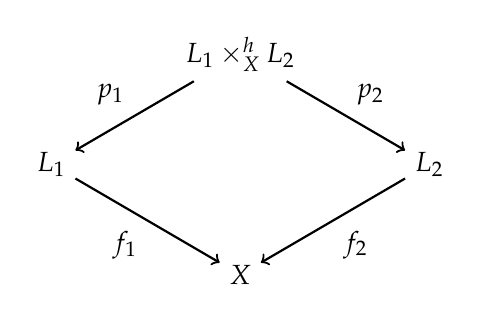
\begin{tikzpicture}[x=1.2cm,y=0.7cm]
        \node (Z) at (0,2) {$L_{1} \times_{X}^{h} L_{2}$};
        \node (L1) at (-2,0) {$L_{1}$};
        \node (L2) at (2,0) {$L_{2}$};
        \node (X) at (0,-2) {$X$};
        
        \draw[->, thick] (Z) -- (L1) node[midway, above left] {$p_{1}$};
        \draw[->, thick] (Z) -- (L2) node[midway, above right] {$p_{2}$};
        \draw[->, thick] (L1) -- (X) node[midway, below left] {$f_{1}$};
        \draw[->, thick] (L2) -- (X) node[midway, below right] {$f_{2}$};
    \end{tikzpicture}
    \caption{The homotopy pullback $L_{1} \times_{X}^{h} L_{2}$ of two Lagrangian morphisms into an $n$-shifted symplectic stack $X$. The concatenation of the isotropic homotopies $h_{1}$ and $h_{2}$ along the pullback square induces the $(n-1)$-shifted symplectic structure on the derived intersection.}
\end{figure}

\section{The AKSZ Construction and Lagrangian Spans}\label{sec:aksz}

We recall the definition of the Betti stack and the transgression morphism. By \cite[Section 1.3]{CHS}, the AKSZ construction defines an extended topological field theory from topological spaces to derived stacks. 

Let $Y$ be a compact oriented topological manifold of dimension $d$. The \bfem{Betti stack} $Y_{B}$ is the locally constant derived stack taking constant value the $\infty$-groupoid associated to the homotopy type of $Y$. The Betti stack $Y_B$ is an $\cO$-compact derived stack \cite[Section 2.1]{PTVV}. For any derived Artin stack $X$, the \bfem{derived mapping stack} $Map(Y, X)$ is the derived space of morphisms from $Y_{B}$ into $X$. 

The AKSZ construction uses a \textit{transgression morphism} to evaluate differential forms on the mapping stack. Let $M$ denote the derived mapping stack $Map(Y, X)$. There is a canonical evaluation morphism $ev \colon Y_{B} \times M \to X$. The derived pullback along the evaluation morphism maps closed 2-forms of degree $n$ on $X$ to closed 2-forms of degree $n$ on the product stack $Y_{B} \times M$.

A topological orientation of the compact manifold $Y$ determines an $\cO$-orientation of dimension $d$ on the $\cO$-compact stack $Y_{B}$ \cite[Section 2.1]{PTVV}. This $\cO$-orientation induces a quasi-coherent integration morphism along the fibers of the projection $\pi \colon Y_{B} \times M \to M$. This integration gives a pushforward morphism on the spaces of closed 2-forms \cite[Definition 2.3]{PTVV}
\[
    \int_{[Y]} \colon \mathcal{A}^{2, \mathrm{cl}}(Y_{B} \times M, n) \to \mathcal{A}^{2, \mathrm{cl}}(M, n-d).
\]

The \bfem{transgression morphism} $\tau$ is defined as the composition of the derived pullback and the integration morphism
\[
    \tau \colon \mathcal{A}^{2, \mathrm{cl}}(X, n) \xrightarrow{ev^*} \mathcal{A}^{2, \mathrm{cl}}(Y_{B} \times M, n) \xrightarrow{\int_{[Y]}} \mathcal{A}^{2, \mathrm{cl}}(M, n-d),
\]leading to the following result:

\begin{theorem}\label{ptvv_a}
Let $X$ be an $n$-shifted symplectic derived stack. The derived mapping stack $Map(Y, X)$ has an $(n-d)$-shifted symplectic structure.
\end{theorem}
\begin{proof}
This theorem is established in \cite[Theorem 2.5]{PTVV}. The transgression morphism $\tau$ maps the $n$-shifted symplectic form $\omega$ on $X$ to an $(n-d)$-shifted closed 2-form $\tau(\omega)$ on the mapping stack. The non-degeneracy of the transgressed form follows from the non-degeneracy of $\omega$ and the Poincaré duality induced by the $\cO$-orientation on $Y_B$.
\end{proof}

An oriented cobordism $W$ between two manifolds $Y_{1}$ and $Y_{2}$ defines a Lagrangian correspondence. The restriction maps to the boundary components define a span of derived mapping stacks
\[
    Map(Y_{1}, X) \leftarrow Map(W, X) \rightarrow Map(Y_{2}, X).
\]
This defines the \bfem{$(\infty, 2)$-category of Lagrangian spans} $Lag_{n}$. The objects of $Lag_{n}$ are $n$-shifted symplectic derived stacks, the 1-morphisms are Lagrangian correspondences, and the 2-morphisms are Lagrangian spans between the correspondences.

\section{Derived Symplectification and Legendrian Morphisms}\label{sec:symplectification}

We define the algebraic structures of derived contact geometry using equivariant descent and the natural symplectic-contact dictionary. 

Let $\cL$ be a line bundle on a derived Artin stack $X$. The \bfem{associated principal $\Gm$-bundle} is defined by the relative spectrum $\widetilde{X} \simeq \mathbf{Spec}_{X}(\bigoplus_{k \in \mathbb{Z}} \cL^{\otimes k})$. The projection morphism $p \colon \widetilde{X} \to X$ has a $\Gm$-action on the fibers. 

The $\Gm$-action on a derived stack induces an auxiliary fiber grading on the derived de Rham complex. Following \cite[Section 2.1.1]{Calaque}, quasi-coherent sheaves on the classifying stack $B\Gm$ are identified with graded complexes. A $\Gm$-action on $\widetilde{X}$ defines a descent to the quotient $[\widetilde{X}/\Gm]$, enhancing the derived de Rham complex to a graded mixed complex. A closed $p$-form $\omega$ on $\widetilde{X}$ has \bfem{weight $w$} if it defines a point in the weight $w$ graded mapping space
\[
    \mathcal{A}^{p, \mathrm{cl}, \{w\}}(\widetilde{X}, n) \simeq \mathrm{Map}_{\epsilon-\mathbf{dg}_{\K}^{gr}}(\K, \mathbf{DR}(\widetilde{X})[n+p](p)\{w\})
\]
where $\epsilon-\mathbf{dg}_{\K}^{gr}$ denotes the \bfem{$\infty$-category of graded mixed $\K$-complexes}, $\K$ denotes the trivial graded mixed complex, and $\{w\}$ denotes the $w$-th shift in the fiber grading.

An \bfem{$n$-shifted contact structure} on $X$ consists of the line bundle $\cL$ and an $n$-shifted symplectic structure $\omega_{\widetilde{X}}$ on $\widetilde{X}$ such that $\omega_{\widetilde{X}}$ has weight 1. The fundamental vector field of the weight 1 $\Gm$-action is the derived analogue of the classical Liouville vector field. The stack quotient of the symplectification recovers the contact structure. In fact, we have:

\begin{theorem}[\cite{IzbudakBerktav}]
Let $\widetilde{X}$ be an $n$-shifted symplectic derived stack equipped with a weight 1 $\Gm$-action. The stack quotient $X \simeq [\widetilde{X} / \Gm]$ admits an $n$-shifted contact structure defined by descent along the principal $\Gm$-bundle projection $p \colon \widetilde{X} \to X$.
\end{theorem}

Let $f \colon L \to X$ be a morphism of derived Artin stacks, with contact target, and $p \colon \widetilde{X} \to X$ the principal $\Gm$-bundle projection. The homotopy pullback of $p$ along $f$ gives a principal $\Gm$-bundle $\widetilde{L} \to L$ and a $\Gm$-equivariant lift $\widetilde{f} \colon \widetilde{L} \to \widetilde{X}$. By an \bfem{(contact) isotropic structure} on $f$, we mean a $\Gm$-equivariant isotropic structure on the lift $\widetilde{f}$ with respect to $\omega_{\widetilde{X}}$.
Such morphism $f \colon L \to X$ is \bfem{Legendrian} if the associated $\Gm$-equivariant lift $\widetilde{f} \colon \widetilde{L} \to \widetilde{X}$ is a Lagrangian morphism. This is the derived analogue of maximally isotropic submanifolds.

\begin{figure}[htbp]
    \centering
    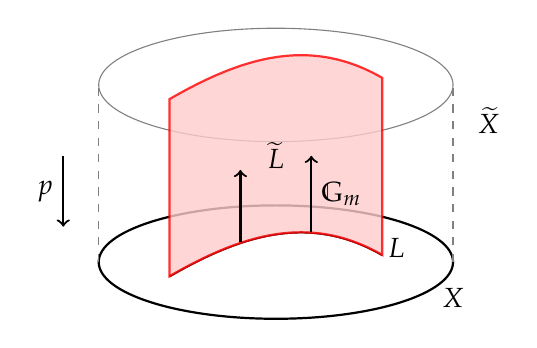
\begin{tikzpicture}[scale=.9]
        \draw[thick] (0,0) ellipse (2.5 and 0.8);
        \node at (2.5, -0.5) {$X$};

        \draw[thick] (-1.5, -0.2) to[out=30, in=150] (1.5, 0.1);
        \node at (1.7, 0.2) {$L$};

        \draw[->, thick] (-3, 1.5) -- (-3, 0.5) node[midway, left] {$p$};

        \draw[dashed, gray] (-2.5, 0) -- (-2.5, 2.5);
        \draw[dashed, gray] (2.5, 0) -- (2.5, 2.5);
        \draw[gray] (0, 2.5) ellipse (2.5 and 0.8);
        \node at (3, 2) {$\widetilde{X}$};

        \filldraw[fill=red!20, draw=red, thick, opacity=0.8] 
            (-1.5, -0.2) to[out=30, in=150] (1.5, 0.1) -- 
            (1.5, 2.6) to[in=30, out=150] (-1.5, 2.3) -- cycle;
        \node at (0, 1.5) {$\widetilde{L}$};

        \draw[->, thick] (0.5, 0.425) -- (0.5, 1.5) node[midway, right] {$\Gm$};
        \draw[->, thick] (-0.5, 0.28) -- (-0.5, 1.3);
    \end{tikzpicture}
    \caption{The Lagrangian lift $\widetilde{L}$ inside the derived symplectification $\widetilde{X}$ over the Legendrian $L$ in the contact base $X$. The fibers are generated by the weight 1 $\Gm$-action modeling the Liouville vector field.}
\end{figure}

\section{Morphism Spaces via Derived Legendrian Intersections}\label{sec:morphisms}

We define the \bfem{objects of $\mathcal{F}_{c}(X)$} to be Legendrian morphisms $f \colon L \to X$. Let $f_1 \colon L_1 \to X$ and $f_2 \colon L_2 \to X$ be objects in $\mathcal{F}_{c}(X)$. The homotopy pullback of the projection $p$ along $f_i$ gives principal $\Gm$-bundles $q_i \colon \widetilde{L}_i \to L_i$. The homotopy pullback gives $\Gm$-equivariant morphisms $\widetilde{f}_i \colon \widetilde{L}_i \to \widetilde{X}$. By the derived Legendrian intersection theorem, the lifts $\widetilde{f}_i$ intersect to form a contact structure on the base.

\begin{theorem}[\cite{IzbudakBerktav}]\label{prev_main}
Let $X$ be an $n$-shifted contact derived stack. Let $f_1 \colon L_1 \to X$ and $f_2 \colon L_2 \to X$ be Legendrian morphisms. The $\Gm$-equivariant Lagrangian lifts $\widetilde{f}_1 \colon \widetilde{L}_1 \to \widetilde{X}$ and $\widetilde{f}_2 \colon \widetilde{L}_2 \to \widetilde{X}$ define a $\Gm$-equivariant $(n-1)$-shifted symplectic structure of weight 1 on the homotopy pullback $\widetilde{L}_1 \times_{\widetilde{X}}^h \widetilde{L}_2$. The descent of this equivariant structure along the principal $\Gm$-bundle defines an $(n-1)$-shifted contact structure on the homotopy pullback $L_1 \times_{X}^h L_2$.
\end{theorem}

The derived intersection of these equivariant Lagrangian structures is computed via a homotopy pullback square and a $\Gm$-equivariant descent diagram.

\begin{figure}[htbp]
    \centering
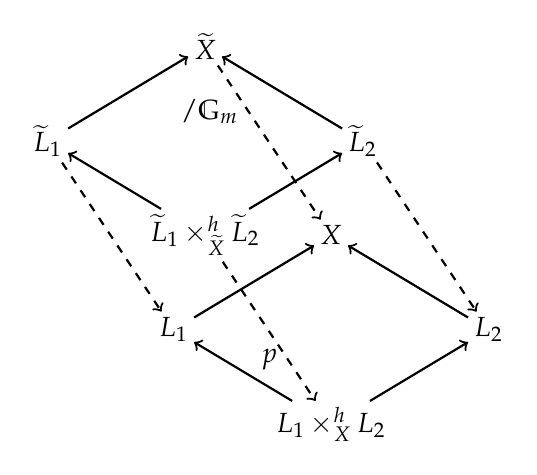
\begin{tikzpicture}[scale=0.8]
    \node[fill=white, inner sep=2pt] (tZ) at (0,0) {$\widetilde{L}_1 \times^h_{\widetilde{X}} \widetilde{L}_2$};
    \node[fill=white, inner sep=2pt] (tL1) at (-2.5, 1.5) {$\widetilde{L}_1$};
    \node[fill=white, inner sep=2pt] (tL2) at (2.5, 1.5) {$\widetilde{L}_2$};
    \node[fill=white, inner sep=2pt] (tX) at (0, 3) {$\widetilde{X}$};

    \node[fill=white, inner sep=2pt] (Z) at (2, -3) {$L_1 \times^h_X L_2$};
    \node[fill=white, inner sep=2pt] (L1) at (-0.5, -1.5) {$L_1$};
    \node[fill=white, inner sep=2pt] (L2) at (4.5, -1.5) {$L_2$};
    \node[fill=white, inner sep=2pt] (X) at (2, 0) {$X$};

    \draw[->, thick, dashed, preaction={draw, white, line width=4pt}] (tX) -- node[pos=0.3, left] {$/\Gm$} (X);
    \draw[->, thick] (tZ) -- (tL1);
    \draw[->, thick] (tZ) -- (tL2);
    \draw[->, thick] (tL1) -- (tX);
    \draw[->, thick] (tL2) -- (tX);

    \draw[->, thick, dashed] (tL1) -- (L1);
    \draw[->, thick, dashed] (tL2) -- (L2);
    
    \draw[->, thick, preaction={draw, white, line width=4pt}] (Z) -- (L1);
    \draw[->, thick, preaction={draw, white, line width=4pt}] (Z) -- (L2);
    \draw[->, thick, preaction={draw, white, line width=4pt}] (L1) -- (X);
    \draw[->, thick, preaction={draw, white, line width=4pt}] (L2) -- (X);
    \draw[->, thick, dashed] (tZ) -- node[pos=0.7, left] {$p$} (Z);
\end{tikzpicture}
    \caption{The homotopy limit diagram. The upper plane is the derived intersection of the $\Gm$-equivariant Lagrangian lifts in the derived symplectification $\widetilde{X}$. The dashed arrows denote the descent via the principal $\Gm$-bundle quotient, giving the derived Legendrian intersection in the contact base $X$.}
\end{figure}

We define the \bfem{1-morphism object $\mathcal{H}om_{\mathcal{F}_{c}(X)}(L_{1}, L_{2})$} as the derived stack $Z \simeq L_{1} \times_{X}^{h} L_{2}$. Hence, the morphism space in the derived Legendrian category is a contact derived stack.

\section{Higher Categories of Lagrangian Spans}\label{sec:higher_categories}

We define the \bfem{composition operations} by defining the derived Legendrian category using iterated spans. Let $L_{0}, L_{1}, L_{2}$ be objects in $\mathcal{F}_{c}(X)$ with their corresponding $\Gm$-equivariant Lagrangian lifts $\widetilde{L}_{0}, \widetilde{L}_{1}, \widetilde{L}_{2}$ in $\widetilde{X}$. By \cite[Section 2]{CHS}, the composition of morphisms in the derived setting is computed by taking the span of homotopy pullbacks.

We consider the triple homotopy pullback of Lagrangian lifts $\widetilde{Z}_{012} \simeq \widetilde{L}_{0} \times_{\widetilde{X}}^{h} \widetilde{L}_{1} \times_{\widetilde{X}}^{h} \widetilde{L}_{2}$. The projection maps from the triple intersection to the pairwise intersections form a span in the $\infty$-category of derived stacks.

\begin{figure}[htbp]
    \centering
    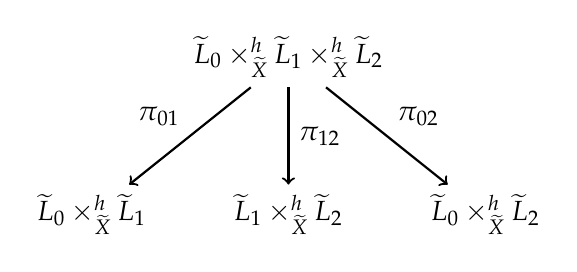
\begin{tikzpicture}[scale=1]
        \node (Z012) at (0,2) {$\widetilde{L}_{0} \times_{\widetilde{X}}^{h} \widetilde{L}_{1} \times_{\widetilde{X}}^{h} \widetilde{L}_{2}$};
        \node (Z01) at (-2.5,0) {$\widetilde{L}_{0} \times_{\widetilde{X}}^{h} \widetilde{L}_{1}$};
        \node (Z12) at (0,0) {$\widetilde{L}_{1} \times_{\widetilde{X}}^{h} \widetilde{L}_{2}$};
        \node (Z02) at (2.5,0) {$\widetilde{L}_{0} \times_{\widetilde{X}}^{h} \widetilde{L}_{2}$};
        
        \draw[->, thick] (Z012) -- (Z01) node[midway, above left] {$\pi_{01}$};
        \draw[->, thick] (Z012) -- (Z12) node[midway, right] {$\pi_{12}$};
        \draw[->, thick] (Z012) -- (Z02) node[midway, above right] {$\pi_{02}$};
    \end{tikzpicture}
    \caption{The derived span defining the composition of morphisms. The triple intersection projects to the pairwise derived intersections, defining the composition map $\mathcal{H}om(L_{1}, L_{2}) \times \mathcal{H}om(L_{0}, L_{1}) \to \mathcal{H}om(L_{0}, L_{2})$.}
\end{figure}

\begin{theorem}\label{thm:span}
The composition operations induced by the Lagrangian spans are well-defined on the contact quotients and satisfy the coherence conditions, making $\mathcal{F}_{c}(X)$ a subcategory of the $(\infty, 2)$-category of spans.
\end{theorem}
\begin{proof}
By \cite[Section 2]{CHS}, shifted symplectic stacks and Lagrangian correspondences form a symmetric monoidal $(\infty, 2)$-category $Lag_{n}$. The pairwise derived intersections $\widetilde{Z}_{ij}$ and the triple derived intersection $\widetilde{Z}_{012}$ are computed via homotopy pullbacks. The stacks $\widetilde{L}_i$ and $\widetilde{X}$ have $\Gm$-actions, and the morphisms between them are $\Gm$-equivariant. Thus, these homotopy limits are computed in the $\infty$-category of $\Gm$-equivariant derived stacks. The projection maps $\pi_{ij} \colon \widetilde{Z}_{012} \to \widetilde{Z}_{ij}$ are the structural morphisms of the homotopy limit cone. Therefore, the projection maps are $\Gm$-equivariant.

By \cite[Section 2.1.1]{Calaque}, a $\Gm$-equivariant morphism between derived stacks induces a $\Gm$-equivariant enhancement on the derived de Rham complexes, preserving the fiber grading over $B\Gm$. Since the projection maps $\pi_{ij}$ are $\Gm$-equivariant, the derived pullback maps $\pi_{ij}^*$ preserve the weight decomposition. Any weight 1 closed 2-form on $\widetilde{Z}_{ij}$ pulls back to a weight 1 closed 2-form on $\widetilde{Z}_{012}$.

The descent along the principal $\Gm$-bundles translates the equivariant span diagram to the contact quotients. The composition sequence thus defines an $(\infty, 2)$-category in $\mathcal{F}_{c}(X)$.

\end{proof}

\section{Topological Cobordisms and Derived Legendrian Surgery}\label{sec:cobordisms}

We define the \textit{Legendrian connected sum} and \textit{surgery} in derived algebraic geometry using the AKSZ construction. 
Consider an oriented topological cobordism $W$ of dimension $d$ with boundary $\partial W \simeq \overline{Y}_{1} \amalg Y_{2}$, which models a topological surgery between $Y_1$ and $Y_2$.

\begin{figure}[htbp]
    \centering
    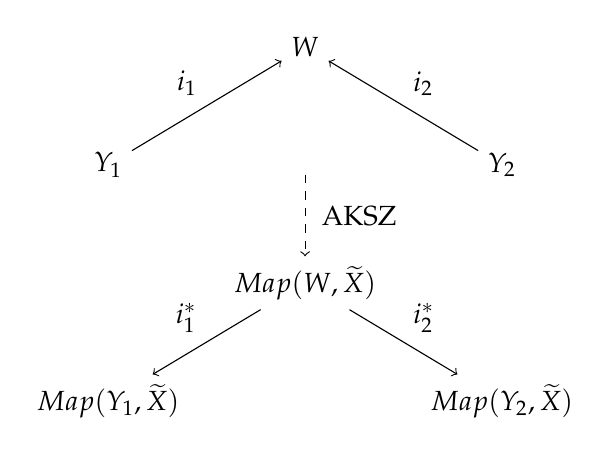
\begin{tikzpicture}[x=2.5cm, y=1.5cm]
        \node (W) at (0, 2) {$W$};
        \node (Y1) at (-1, 1) {$Y_1$};
        \node (dummy) at (0, 1) {};
        \node (Y2) at (1, 1) {$Y_2$};
        \node (MapW) at (0, 0) {$Map(W, \widetilde{X})$};
        \node (MapY1) at (-1, -1) {$Map(Y_{1}, \widetilde{X})$};
        \node (MapY2) at (1, -1) {$Map(Y_{2}, \widetilde{X})$};

        \draw[->] (Y1) -- node[above left] {$i_1$} (W);
        \draw[->] (Y2) -- node[above right] {$i_2$} (W);
        \draw[->, dashed] (dummy) -- node[right] {\ AKSZ} (MapW);
        \draw[->] (MapW) -- node[above left] {$i_1^*$} (MapY1);
        \draw[->] (MapW) -- node[above right] {$i_2^*$} (MapY2);
    \end{tikzpicture}
    \caption{The topological cobordism $W$ mapped to a Lagrangian span via the AKSZ functor $\mathcal{Z} _{\widetilde{X}}$. The topological inclusions of the boundary components induce the projection morphisms of the Lagrangian span.}
\end{figure}

\begin{proposition}\label{prop:equiv_mapping_stack}
The mapping stack $Map(W, \widetilde{X})$ has a $\Gm$-equivariant Lagrangian structure over the product stack $Map(Y_{1}, \widetilde{X}) \times Map(Y_{2}, \widetilde{X})$.
\end{proposition}
\begin{proof}
We assign the trivial $\Gm$-action to the Betti stack $W_B$ \cite[Section 2.1]{PTVV}. The Betti stack $W_B$ is an $\cO$-compact derived stack. The derived mapping stack functor
\[
    \mathbb{R}Map(W_B, -) \colon \mathbf{dSt} \to \mathbf{dSt}
\]
is a right adjoint and preserves limits. A $\Gm$-action on $\widetilde{X}$ is formalized as an object in the functor $\infty$-category $\mathrm{Fun}(B\Gm, \mathbf{dSt})$. The functor $\mathbb{R}Map(W_B, -)$ operates pointwise on this functor category, inducing a $\Gm$-action on $Map(W, \widetilde{X})$. The topological inclusions $i \colon \partial W \to W$ induce morphisms of Betti stacks $i_B \colon (\partial W)_B \to W_B$ in the $\infty$-category of derived stacks \cite[Section 2.1]{PTVV}. 

The functoriality yields $\Gm$-equivariant restriction maps and an evaluation morphism
\begin{align*}
    i^* &\colon Map(W, \widetilde{X}) \to Map(\partial W, \widetilde{X}) \\
    ev_W &\colon W_B \times Map(W, \widetilde{X}) \to \widetilde{X}
\end{align*}
The boundary inclusions and restriction maps commute with the evaluation morphisms in the $\Gm$-equivariant evaluation diagram
\begin{center}
    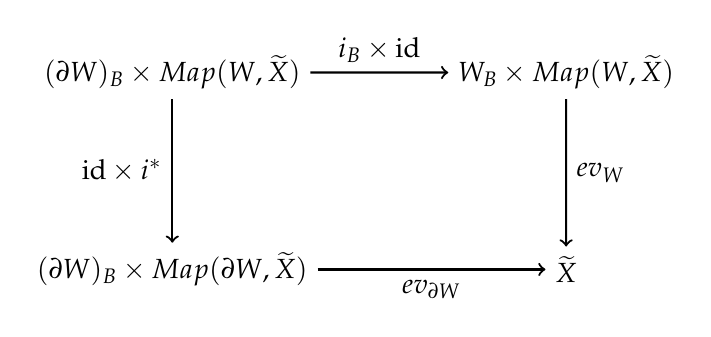
\begin{tikzpicture}[scale=1.25]
        \node (dWMapW) at (0, 2) {$(\partial W)_B \times Map(W, \widetilde{X})$};
        \node (WMapW) at (4, 2) {$W_B \times Map(W, \widetilde{X})$};
        \node (dWMapdW) at (0, 0) {$(\partial W)_B \times Map(\partial W, \widetilde{X})$};
        \node (X) at (4, 0) {$\widetilde{X}$};
        
        \draw[->, thick] (dWMapW) -- (WMapW) node[midway, above] {$i_B \times \mathrm{id}$};
        \draw[->, thick] (dWMapW) -- (dWMapdW) node[midway, left] {$\mathrm{id} \times i^*$};
        \draw[->, thick] (WMapW) -- (X) node[midway, right] {$ev_W$};
        \draw[->, thick] (dWMapdW) -- (X) node[midway, below] {$ev_{\partial W}$};
    \end{tikzpicture}
\end{center}
Applying the derived pullback and the relative $\cO$-orientation functional to this diagram generates the isotropic null-homotopy $h$.

A Lagrangian correspondence requires an isotropic null-homotopy $h$ between zero and the pullback of the boundary symplectic forms. This null-homotopy is represented by the path
\[
    h \colon 0 \sim (i^*)^* (\omega_{\partial W}).
\]
The relative $\cO$-orientation on the pair $(W_B, \partial W_B)$ defines this null-homotopy \cite[Section 2.1]{PTVV}. The relative orientation functional operates on the fiber of the restriction map
\[
    C(W_B, \cO_{W_B}) \to C(\partial W_B, \cO_{\partial W_B}).
\]
Since $W_B$ and $\partial W_B$ carry trivial $\Gm$-actions, this fiber complex has weight 0. The induced isotropic null-homotopy $h$ is a path within the weight 1 graded component of the derived de Rham complex. The Poincaré-Lefschetz duality of the relative $\cO$-orientation guarantees the non-degeneracy of this isotropic structure. This establishes the $\Gm$-equivariant Lagrangian correspondence.
\end{proof}

\begin{theorem}\label{thm:surgery}
The topological cobordism descends to a derived Legendrian correspondence representing a 1-morphism in the $(\infty, 2)$-category of Legendrian correspondences.
\end{theorem}

\begin{proof}
By Proposition \ref{prop:equiv_mapping_stack}, the topological cobordism yields a $\Gm$-equivariant Lagrangian span between the mapping stacks $Map(Y_{1}, \widetilde{X})$ and $Map(Y_{2}, \widetilde{X})$. The stack quotient descends this span to a derived Legendrian correspondence between the contact mapping stacks $X_{Y_1}$ and $X_{Y_2}$. Therefore, this defines a 1-morphism in the global category of contact stacks.

\end{proof}

\section{Proof of Main Results}\label{sec:proof}

\noindent We verify the three properties of the derived Legendrian category $\mathcal{F}_{c}(X)$ sequentially.

\begin{enumerate}\itemsep=8pt
    \item We define the \bfem{objects} of $\mathcal{F}_{c}(X)$ to be the Legendrian morphisms $f \colon L \to X$.
    \item Let $f_{1} \colon L_{1} \to X$ and $f_{2} \colon L_{2} \to X$ be Legendrian objects in $\mathcal{F}_{c}(X)$. 
    By Theorem \ref{prev_main}, the homotopy pullback $\widetilde{Z} \simeq \widetilde{L}_{1} \times_{\widetilde{X}}^{h} \widetilde{L}_{2}$ of their equivariant Lagrangian lifts has a $\Gm$-equivariant $(n-1)$-shifted symplectic structure of weight 1.
    By \cite[Theorem 3.7]{IzbudakBerktav}, taking the stack quotient of this derived intersection by the $\Gm$-action yields the stack $Z \simeq [\widetilde{Z}/\Gm]$. This quotient has an $(n-1)$-shifted contact structure. We define the \bfem{morphism space} $\mathcal{H}om_{\mathcal{F}_{c}(X)}(L_{1}, L_{2})$ as $Z$.
    \item Let $L_{0}, L_{1}, L_{2}$ be objects in $\mathcal{F}_{c}(X)$.
    By Theorem \ref{thm:span}, the triple homotopy pullback $\widetilde{Z}_{012}$ provides a span of Lagrangian correspondences projecting onto the pairwise intersections. This span commutes with the weight 1 $\Gm$-action. The equivariant descent translates this span to a \bfem{composition} sequence in the contact base. From \cite[Theorem 2.7]{CHS}, this sequence satisfies the coherence conditions of $Lag_{n}$.
\end{enumerate}This completes the proof of Theorem \ref{thm:A}. From that, we have an immediate corollary:

\begin{corollary}\label{defn:Leg_n}
We promote the collection of $n$-shifted contact derived stacks into a global $(\infty, 2)$-category, written $Leg_n$, by descending the $\Gm$-equivariant $(\infty, 2)$-category of Lagrangian spans. \begin{itemize}
    \item The \emph{objects} of this $(\infty, 2)$-category are $n$-shifted contact derived stacks.
    \item A \emph{1-morphism} between contact stacks $X_{1}$ and $X_{2}$ is a derived Legendrian correspondence formulated as a span \[ X_{1} \leftarrow L \rightarrow X_{2}. \]
This Legendrian correspondence is defined such that the associated principal $\Gm$-bundles form a $\Gm$-equivariant Lagrangian span $\widetilde{X}_{1} \leftarrow \widetilde{L} \rightarrow \widetilde{X}_{2}$ between the derived symplectifications.
    \item Let $L$ and $L'$ be two Legendrian correspondences between $X_{1}$ and $X_{2}$. A \emph{2-morphism} from $L$ to $L'$ is a Legendrian span \[ L \leftarrow M \rightarrow L' \] commuting with the projections to $X_{1}$ and $X_{2}$. This 2-morphism is defined such that the equivariant lift $\widetilde{M}$ forms a $\Gm$-equivariant Lagrangian span between the Lagrangian correspondences $\widetilde{L}$ and $\widetilde{L}'$.
\end{itemize} Call $Leg_n$ the \bfem{$(\infty,2)$-category  of Legendrian correspondences.}  
\end{corollary}

\section{Applications to Derived Moduli Stacks}\label{sec:applications}

We apply the derived Legendrian category $\mathcal{F}_{c}(X)$ to specific derived moduli spaces. The composition operations, endomorphism algebras, and functoriality define the non-commutative and shifted geometry of these spaces.

\subsection{Convolution of Derived Discriminant Loci}
Let $L$ be a smooth $\K$-scheme. The classical 1-jet space $(J^1(L), \xi_{jet})$ carries a canonical $0$-shifted contact structure. A regular function $f \in \cO(L)$ defines a Legendrian embedding $L_F$ of $L$ into $J^1(L)$ via the 1-jet prolongation map $j^1f \colon p \mapsto (p, f(p), d_{dR}f_p)$. Let $L_0$ denote the Legendrian corresponding to the 1-jet of the zero function, $j^1 0$. 

The \bfem{derived discriminant locus} $\Delta\mathrm{loc}(f)$ is defined by the homotopy pullback
\[
    \Delta\mathrm{loc}(f) \simeq L_F \times_{J^1(L)}^h L_0.
\]
This derived intersection captures the contact analogue of the derived critical locus, representing the derived space of points where both $f=0$ and $df=0$. By Theorem \ref{prev_main}, this locus inherits a $(-1)$-shifted contact structure. The space $\Delta\mathrm{loc}(f)$ represents the morphism space $\mathcal{H}om_{\mathcal{F}_{c}(J^1(L))}(L_F, L_0)$ in our category. 
The categorical structure of $\mathcal{F}_{c}(J^1(L))$ equips this intersection with higher composition operations, leading to: 
\begin{proposition}\label{prop: disclocus}
 Given two regular functions $f_1$ and $f_2$, the composition span defined in Theorem \ref{thm:span} yields a derived convolution map
\[
    \mathcal{H}om(L_{F_1}, L_0) \times \mathcal{H}om(L_{F_2}, L_{F_1}) \to \mathcal{H}om(L_{F_2}, L_0).
\]   
\end{proposition}
This spans the product $\Delta\mathrm{loc}(f_1) \times (L_{F_2} \times_{J^1(L)}^h L_{F_1})$ into $\Delta\mathrm{loc}(f_2)$. Consequently, the derived Legendrian category provides a convolution algebra for derived discriminant loci as a geometric analogue of the composition of microlocal kernels over derived stacks in the sense of Guillermou and Schapira \cite{GuillermouSchapira}.

\subsection{The Deformation Algebra of the Nilpotent Cone}
Let $C$ be a smooth proper curve over $\K$ and let $G$ be a reductive algebraic group. The derived moduli stack $P\mathrm{Higgs}_G(C)$ of projective Higgs bundles admits a $0$-shifted contact structure. The projectivized derived nilpotent cone $\mathbb{P}\mathcal{N}$ is a Legendrian substack of $P\mathrm{Higgs}_G(C)$ \cite[Theorem 4.1]{IzbudakBerktav}. Therefore $\mathbb{P}\mathcal{N}$ defines an object in the derived Legendrian category $\mathcal{F}_{c}(P\mathrm{Higgs}_G(C))$.

We define the endomorphism space of the projectivized nilpotent cone as the derived intersection
\[
\mathcal{E}nd(\mathbb{P}\mathcal{N}) \simeq \mathcal{H}om_{\mathcal{F}_{c}(P\mathrm{Higgs}_G(C))}(\mathbb{P}\mathcal{N}, \mathbb{P}\mathcal{N}).
\]
\begin{figure}[htbp]
    \centering
    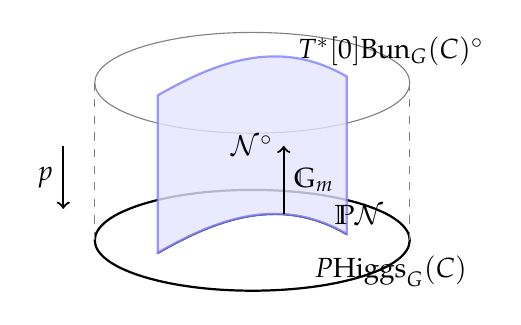
\begin{tikzpicture}[scale=.8]
        \draw[thick] (0,0) ellipse (2.5 and 0.8);
        \node at (2.2, -0.5) {$P\mathrm{Higgs}_G(C)$};

        \draw[thick] (-1.5, -0.2) to[out=30, in=150] (1.5, 0.1);

        \draw[->, thick] (-3, 1.5) -- (-3, 0.5) node[midway, left] {$p$};

        \draw[dashed, gray] (-2.5, 0) -- (-2.5, 2.5);
        \draw[dashed, gray] (2.5, 0) -- (2.5, 2.5);
        \draw[gray] (0, 2.5) ellipse (2.5 and 0.8);
        \node at (2.2, 3) {$T^*[0]\mathrm{Bun}_G(C)^\circ$};

        \filldraw[fill=blue!10, draw=blue!50, thick, opacity=0.8] 
            (-1.5, -0.2) to[out=30, in=150] (1.5, 0.1) -- 
            (1.5, 2.6) to[in=30, out=150] (-1.5, 2.3) -- cycle;
        \node at (0, 1.5) {$\mathcal{N}^\circ$};
        \node at (1.7, 0.4) {$\mathbb{P}\mathcal{N}$};


        \draw[->, thick] (0.5, 0.425) -- (0.5, 1.5) node[midway, right] {$\Gm$};
    \end{tikzpicture}
    \caption{\small The Legendrian inclusion of the projectivized nilpotent cone $\mathbb{P}\mathcal{N}$ into the derived moduli stack of projective Higgs bundles. The Legendrian condition is equivalent to the equivariant lift $\mathcal{N}^\circ$ forming a Lagrangian sub-moduli stack in the derived symplectification.}
\end{figure}
The projectivized derived nilpotent cone $\mathbb{P}\mathcal{N}$ is therefore an object in the derived Legendrian category $\mathcal{F}_{c}(P\mathrm{Higgs}_G(C))$, and hence we get the following proposition. %We consider its endomorphism space \[ \mathcal{E}nd(\mathbb{P}\mathcal{N}) \simeq \mathcal{H}om_{\mathcal{F}_{c}(P\mathrm{Higgs}_G(C))}(\mathbb{P}\mathcal{N}, \mathbb{P}\mathcal{N}). \]

\begin{proposition}\label{prop: nilpotentcone}
The categorical composition in $\mathcal{F}_{c}(P\mathrm{Higgs}_G(C))$ equips the homotopy pullback
\[
    \mathbb{P}\mathcal{N} \times_{P\mathrm{Higgs}_G(C)}^h \mathbb{P}\mathcal{N}
\]
with an $A_\infty$-algebra structure in the $(\infty, 2)$-category of Legendrian correspondences.
\end{proposition}
\begin{proof}
Since $\mathbb{P}\mathcal{N}$ is an object in $\mathcal{F}_{c}(P\mathrm{Higgs}_G(C))$, Theorem \ref{thm:span} yields a derived span of Legendrian correspondences. This span induces a composition map
\[
    \mathcal{E}nd(\mathbb{P}\mathcal{N}) \times \mathcal{E}nd(\mathbb{P}\mathcal{N}) \to \mathcal{E}nd(\mathbb{P}\mathcal{N})
\]
in the contact base. The coherence conditions of the $(\infty, 2)$-category $Lag_{n}$ induce higher associativity homotopies for this composition operation. Thus, the endomorphism space $\mathcal{E}nd(\mathbb{P}\mathcal{N})$ acquires the structure of an $A_\infty$-algebra. Furthermore, Theorem \ref{prev_main} dictates that $\mathcal{E}nd(\mathbb{P}\mathcal{N})$ inherits a $(-1)$-shifted contact structure. This algebra governs the non-commutative deformation theory of the projectivized nilpotent cone.

\end{proof}

\subsection{Topological Field Theories and Functoriality}
Let $Y$ be a closed oriented topological manifold of dimension $d-1$. Let $\widetilde{X}$ be a $k$-shifted symplectic derived stack equipped with a weight 1 $\Gm$-action. By Theorem \ref{ptvv_a}, the derived mapping stack $Map(Y, \widetilde{X})$ has a $(k-d+1)$-shifted symplectic structure. Since the fundamental class integration commutes with the target $\Gm$-action, $Map(Y, \widetilde{X})$ has a weight 1 $\Gm$-action. The stack quotient $X_Y \simeq [Map(Y, \widetilde{X}) / \Gm]$ has a $(k-d+1)$-shifted contact structure.

Let $\mathrm{Bord}_d$ denote the symmetric monoidal $\infty$-category of oriented $d$-dimensional cobordisms \cite[Section 1.2]{CHS}. Let $Leg_{n}$ denote the global $(\infty, 2)$-category of $n$-shifted contact derived stacks introduced in Corollary \ref{defn:Leg_n}. Then we provide:

\begin{proposition} \label{prop:AKSZ}
The AKSZ construction extends to a symmetric monoidal $\infty$-functor \[ \mathcal{Z}_{c} \colon \mathrm{Bord}_d \to Leg_{k-d+1} \] capturing derived Legendrian surgery.
\end{proposition}
\begin{proof}
We construct the functor $\mathcal{Z}_{c}$ by combining the classical AKSZ functor with equivariant descent. To a closed oriented $(d-1)$-manifold $Y$, the functor assigns the $(k-d+1)$-shifted contact stack $X_Y \simeq [Map(Y, \widetilde{X}) / \Gm]$. To an oriented $d$-dimensional cobordism $W$ between $Y_1$ and $Y_2$, the functor assigns the derived stack $L_W \simeq [Map(W, \widetilde{X}) / \Gm]$. By Proposition \ref{prop:equiv_mapping_stack}, $Map(W, \widetilde{X})$ forms a $\Gm$-equivariant Lagrangian span between $Map(Y_1, \widetilde{X})$ and $Map(Y_2, \widetilde{X})$. Its descent $L_W$ thus defines a Legendrian correspondence between $X_{Y_1}$ and $X_{Y_2}$, representing a 1-morphism in $Leg_{k-d+1}$.

The topological gluing of cobordisms $W_1 \cup_Y W_2$ corresponds to the homotopy pullback of the mapping stacks over $Map(Y, \widetilde{X})$. By Theorem \ref{thm:span}, this equivariant pullback descends to the categorical composition of Legendrian spans in $Leg_{k-d+1}$. Therefore, $\mathcal{Z}_{c}$ preserves the composition structure of cobordisms and defines an $\infty$-functor.

\end{proof}

This functoriality provides a categorical framework for \bfem{derived Legendrian surgery}. The geometric gluing of cobordisms maps directly to the associative composition operation in the global contact category. This evaluates the gluing of moduli problems on $d$-manifolds as the composition of local Legendrian boundary conditions.

\subsection{Outlook: Towards Derived Contact Surgery}
Our construction of the derived Legendrian category $\mathcal{F}_{c}(X)$ and the formulation of topological cobordisms as Legendrian spans (Theorem \ref{thm:surgery}) provide the necessary setup to define surgery operations directly on contact stacks. In classical contact topology, Weinstein surgery is performed by attaching isotropic and Legendrian handles. In the derived setting, a \bfem{derived contact surgery} along a Legendrian morphism $f \colon L \to X$ should correspond to a specific quotient of the derived symplectification of $X$, modified by the Lagrangian span associated with the surgery cobordism. 

Future work will explore how to compute the effect of such surgeries on the resulting shifted contact structures using this $(\infty, 2)$-categorical framework. In particular, we aim to establish how the derived mapping stacks of surgery traces behave under $\Gm$-equivariant descent. This will yield a systematic method for constructing new shifted contact moduli spaces from existing ones via categorical gluing.

\section*{Acknowledgements}
The first author (E.\.{I}.) wishes to express his deepest gratitude to the second author (K.\.{I}.B.) for his invaluable mentorship, generous guidance, and continuous support. The central question addressed in this paper concerning the construction of a derived Legendrian category was explicitly posed by K.\.{I}.B., whose core ideas and foundational work in derived contact geometry provide the overarching conceptual framework for this text. The specific categorical constructions and the proofs of the main theorems were subsequently developed by E.\.{I}. 

Both authors warmly thank the Higher Structures Group in the Math  Department at Middle East Technical University for fostering a stimulating research environment.

\begin{thebibliography}{9}
\bibitem{IzbudakBerktav} E. \.{I}zbudak and K. \.{I}. Berktav, \bfem{Equivariant Quotients of Derived Symplectic Spaces and Legendrian Intersection Theorem}, 2026.      arXiv:2605.08394
\bibitem{PTVV} T. Pantev, B. To\"{e}n, M. Vaqui\'{e}, G. Vezzosi, \bfem{Shifted Symplectic Structures}, Publ. Math. Inst. Hautes \'{E}tudes Sci. 117 (2013), 271-328.
\bibitem{Calaque} D. Calaque, \bfem{Shifted cotangent stacks are shifted symplectic}, Ann. Fac. Sci. Toulouse Math. 28 (2019), no. 1, 67-90.
\bibitem{CHS} D. Calaque, R. Haugseng, C. Scheimbauer, \bfem{The AKSZ Construction in Derived Algebraic Geometry as an Extended Topological Field Theory}, arXiv:2108.02473, 2022.
 \bibitem{Berktav1}
  K. \.{I}. Berktav,
  \bfem{Shifted Contact Structures and Their Local Theory}, Ann. Fac.
  Sci. Toulouse, Math., Serie 6, Vol. 33(4): 1019-1057, 2024.

  \bibitem{Berktav2}
  K. \.{I}. Berktav,
  \bfem{On shifted contact derived Artin stacks},
  Higher Structures 9(2):103--135, 2025

  \bibitem{GuillermouSchapira}
S. Guillermou and P. Schapira, \bfem{Microlocal Theory of Sheaves and
Tamarkin's Non Displaceability Theorem}, in: \textit{Homological Mirror
Symmetry and Tropical Geometry}, Springer International Publishing,
Cham, 2014, pp. 43--85.
  \bibitem{Ginzburg2000}
V. Ginzburg, \bfem{The global nilpotent variety is Lagrangian},
arXiv:alg-geom/9704005, 2000.
\end{thebibliography}

\end{document}
